\subsection{Erweiterung durch verschiedene Sensoren}\label{ss:sensoren}

Eine Erweiterungsmöglichkeit ist die Ergänzung verschiedener Sensoren. 
Durch ein Mikrophon können ungewöhnliche Geräusche aufgezeichnet werden. Diese können von Einbruchsversuchen an einer Tür oder durch eine zerbrechende Scheibe entstehen. Eine großer Vorteil eines Mikrophons ist, das auch jegliche Kommunikation der Einbrecher aufgezeichnet werden kann. So kann ebenfalls entschieden werden, ob es sich um einen Einbrecher handelt, oder ob Verwandtschaft mit einem Ersatzschlüssel die Wohnung betreten hat.\\

Durch Bewegungsmelder werden häufig Beleuchtungen, in diesem Szenario kann er jedoch zur Einbruchserkennung verwendet werden: Falls sich etwas bewegt, jedoch niemand zu hause sein sollte, wird ein Alarm ausgelöst. 
Da die Überwachung durch Ultraschall oder Infrarot geschieht, kann es im Raum auch dunkel sein.\\

Eine weitere Möglichkeit ist das Ergänzen einer Kamera. Diese kann entweder als Bewegungsmelder eingesetzt werden, oder Bilder und Videos der Wohnung aufnehmen. Im Falle eines Einbruchs kann so der Täter direkt photographiert werden. Dies  Ermöglicht eine gezielte strafrechtliche Verfolgung. Die Kamera kann jedoch auch auf Wunsch des Wohnungsbesitzers Bild- oder Videomaterial aufzeichnen, dass über das Internet einsehbar ist. Auf diese Weise kann man einen Blick in die Wohnung werfen, ohne anwesend zu sein.

Die verschiedenen Sensoren können beispielsweise an einen Raspberry Pi angeschlossen werden, der die Eingangssignale überwacht, und bei ungewöhnlichen Werten anschlägt.

\begin{figure}[H] 
	\centering
	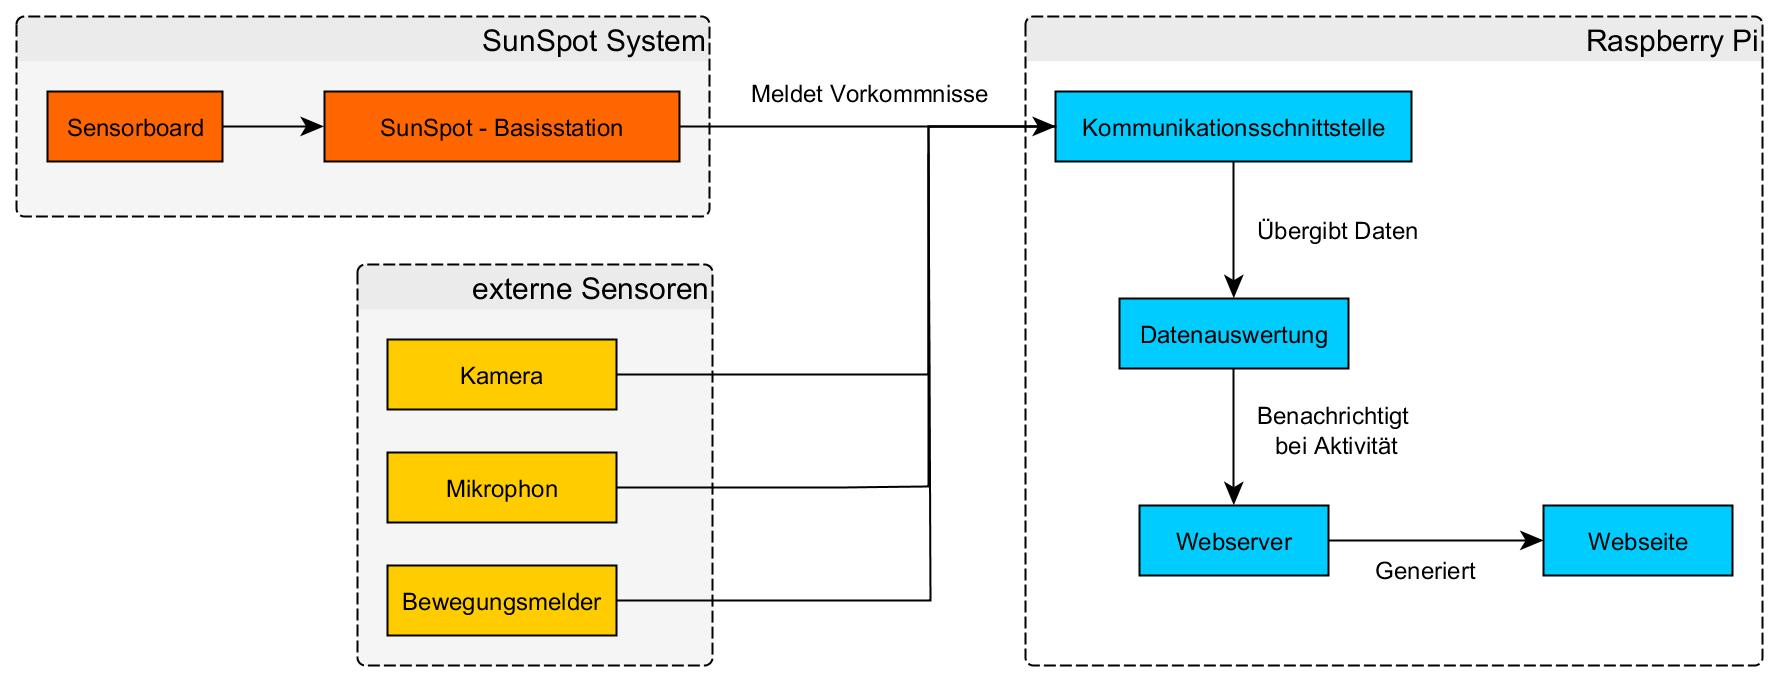
\includegraphics[scale=0.22]{Bilder/extSensor}
	\caption{Aufbau eines Sensornetzes mithilfe eines Raspberry Pis}
	\label{f:extSensor}
\end{figure}